\documentclass[tikz,border=8pt]{standalone}
\begin{document}
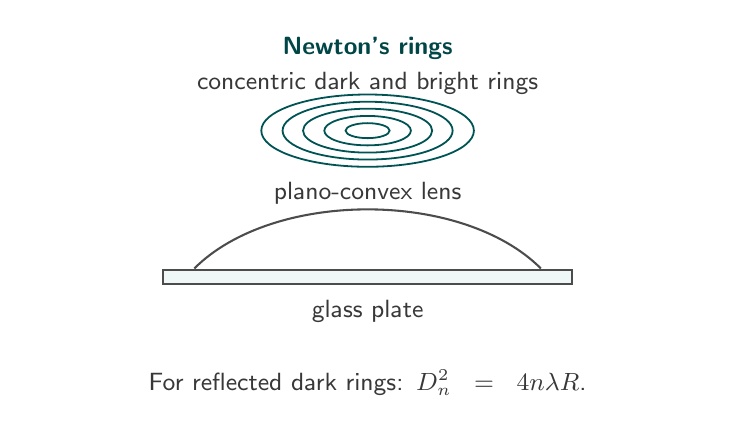
\begin{tikzpicture}[
  line/.style={draw=black!70,line width=0.75pt},
  label/.style={font=\sffamily\small,text=black!78},
  title/.style={font=\sffamily\bfseries\small,text=teal!55!black},
]
\node[title] at (0,3.0) {Newton's rings};
\draw[line,fill=teal!6] (-2.6,0) rectangle (2.6,0.18);
\draw[line] (-2.2,0.2) .. controls (-1.2,1.2) and (1.2,1.2) .. (2.2,0.2);
\node[label] at (0,-0.35) {glass plate};
\node[label] at (0,1.15) {plano-convex lens};
\foreach \r in {0.28,0.55,0.82,1.08,1.35}{
  \draw[teal!65!black,line width=0.65pt] (0,1.95) ellipse ({\r} and {0.34*\r});
}
\node[label] at (0,2.55) {concentric dark and bright rings};
\node[label,align=center,text width=8.4cm] at (0,-1.25)
  {For reflected dark rings: $D_n^2=4n\lambda R$.};
\end{tikzpicture}
\end{document}
